% !TeX program = pdflatex
% !TeX encoding = UTF-8
% !TeX spellcheck = pt_BR
\documentclass[
  article,
  11pt,
  a4paper,
  english,
  brazil,
  sumario=tradicional]{abntex2}
\usepackage{lmodern}			% Usa a fonte Latin Modern
\usepackage[T1]{fontenc}		% Selecao de codigos de fonte.
\usepackage[utf8]{inputenc}		% Codificacao do documento (conversão automática dos acentos)
\usepackage{indentfirst}		% Indenta o primeiro parágrafo de cada seção.
\usepackage{nomencl} 			% Lista de simbolos
\usepackage{color}				% Controle das cores
\usepackage{graphicx}			% Inclusão de gráficos
\usepackage{microtype} 			% para melhorias de justificação

\usepackage{csquotes}
% ---
% Pacotes de citações
% ---
\usepackage[brazilian,hyperpageref]{backref}	 % Paginas com as citações na bibl
\usepackage[alf]{abntex2cite}	% Citações padrão ABNT
% ---

% ---
% Configurações do pacote backref
% Usado sem a opção hyperpageref de backref
\renewcommand{\backrefpagesname}{Citado na(s) página(s):~}
% Texto padrão antes do número das páginas
\renewcommand{\backref}{}
% Define os textos da citação
\renewcommand*{\backrefalt}[4]{
  \ifcase #1 %
  Nenhuma citação no texto.%
  \or
  Citado na página #2.%
  \else
  Citado #1 vezes nas páginas #2.%
  \fi}%
% ---

% Para fórmulas matemáticas
\usepackage{amsmath}
\usepackage{amssymb}
\usepackage{mathtools}

% Diretório padrão para figuras
\graphicspath{ {images/} }

\hypersetup{
  %hidelinks,   % Comente aqui para exibir os links
  colorlinks, % Descomente esse se comentar o de cima
  linkcolor={red!50!black},
  citecolor={blue!50!black},
  urlcolor={blue!80!black}
}

\usepackage[pdftex,dvipsnames,table,xcdraw]{xcolor}

% Para setas usadas em fórmulas dos grafos
\usepackage{MnSymbol}

% ---
% Altera as margens padrões
% ---
\setlrmarginsandblock{3cm}{3cm}{*}
\setulmarginsandblock{3cm}{3cm}{*}
\checkandfixthelayout
% ---

% --- 
% Espaçamentos entre linhas e parágrafos 
% --- 

% O tamanho do parágrafo é dado por:
\setlength{\parindent}{1.3cm}

% Controle do espaçamento entre um parágrafo e outro:
\setlength{\parskip}{0.2cm}  % tente também \onelineskip

% Espaçamento simples
\SingleSpacing

% Titulo e coisas para cabeçalho
\title{Identificação de Carreiras utilizando Detecção de Comunidades}
\author{Ronie Uliana}

\begin{document}

% Seleciona o idioma do documento (conforme pacotes do babel)
%\selectlanguage{english}
\selectlanguage{brazil}

% Retira espaço extra obsoleto entre as frases.
\frenchspacing

\maketitle

\begin{abstract}
Resumo vai aqui
\end{abstract}

%===================================
\section{Introdução}
%===================================

Carreira profissional e trajetória pessoal

O objetivo desse trabalho é identificar carreiras profissionais a partir de uma rede que representa a movimentação de profissionais entre ocupações.

Essa rede foi gerada pela empresa VAGAS Tecnologia e é explicada em detalhes na Seção~\ref{sec:mapa}. Nela, cada nó representa uma ocupação profissional, as conexões são direcionadas e representam o número de profissionais que passou de uma ocupação para outra em sua trajetória pessoal.



Foram utilizados algoritmos de detecção de comunidades para identificação das carreiras

O modelo ideal de detecção de comunidade permite que um nó faça parte de mais de uma comunidade, desse jeito uma ocupação pode fazer parte de mais de uma carreira. Isso acontece em dois casos: \enquote{Gerente de Projeto} que é uma ocupação homônima para várias carreiras (vide imagem) e \enquote{a-definir} que faz a \enquote{ponte} entre carreiras distintas.

%===================================
\section{Carreira, Fronteira e Permeabilidade} \label{sec:carreira}
%===================================

Segundo~\citeonline{Arthur1989-rn}, carreira é \foreignquote{english}{uma sequência evolutiva da experiência profissional de uma pessoa no tempo}\footnote{No original: \enquote{an evolving sequence of person's work experience over time}.}.

Apesar das discussões sobre as mudanças nos modelos de carreira, passando de um modelo linear e centrado na organização para um modelo centrado do indivíduo, as definições de carreira são frequentemente associadas à progressão ou sequência profissional do indivíduo~\cite{Baruch2004-oy,Sullivan2009-xb,Bendassolli2009-bg}.

Para os fins desse trabalho, define-se carreira como \textit{a sequência de ocupações pela qual um indivíduo passa em sua vida profissional}. Essa definição é similar à de \citeonline{Arthur1989-rn}, porém, limita a abrangência da definição e a torna mais concreta. Isso permite uma análise menos subjetiva, uma vez que ocupações profissionais podem ser extraídas objetivamente de currículos e analisadas quantitativamente. No entanto, ela se torna mais limitada, já que essa definição exclui aspectos psicológicos ou sociais.

Esse trabalho empresta o conceito de \enquote{fronteiras de carreira} (\textit{career boundaries}) de \citeonline{Gunz2007-hr} para dar significado ao trabalho.

Segundo os autores, a definição de ocupação profissional é subjetiva, sendo um construto psicológico e pessoal. No entanto, quando um grupo suficientemente grande de pessoas entra em \textit{consenso} sobre o que é uma ocupação, ela passa a ser objetiva. Como exemplo, a ocupação de \enquote{Arquiteto de Software} é um conceito que depende da concepção de quem exerce a profissão, de quem contrata o cargo e de outros agentes interessados na ocupação. Quando vários profissionais e recrutadores (entre outros agentes) criam um certo consenso sobre o que faz ou não um Arquiteto de Software, esse consenso, ainda que impreciso, define suas fronteiras. Essa definição cria a ocupação de maneira objetiva.

A fronteira de carreira significa que a mudança entre ocupações não pode ser realizada livremente. Por exemplo, um profissional precisa de graduação especializada antes de poder se mover da ocupação de \enquote{Auxiliar de Jardinagem} para \enquote{Médico}, por outro lado, a barreira para mesmo profissional exercer a ocupação de \enquote{Jardineiro} se limita à experiência. É possível perceber que as barreiras não são simétricas, em um momento de crise é mais simples para uma \enquote{Engenheiro} tornar-se um \enquote{Corretor de Imóveis} do que o contrário.

Essas barreiras não se limitam ao conhecimento, quaisquer dificuldades na movimentação podem criar fronteiras. Por exemplo, alguém morando em um grande centro urbano dificilmente exerceria a ocupação de \enquote{Agricultor} sem mover-se para o campo. Um \enquote{Diretor Financeiro} precisaria adequar seu padrão de vida antes de uma transição para uma ocupação com ganhos mais modestos. Uma profissão que está desaparecendo, como \enquote{Contínuo} possui barreiras mais altas do que uma nascendo, como \enquote{Analista de Experiência do Usuário}.

A permeabilidade diretamente relacionada à dificuldade em se cruzar uma fronteira.

Observando-se a movimentação profissional é possível inferir permeabilidade entre ocupações. Quanto mais profissionais se movem entre elas, mais permeáveis são suas fronteiras. Esse tipo de observação não permite analisar a natureza da barreira, ou seja, o que torna a movimentação fácil ou difícil, mas permite dizer seu grau de permeabilidade.

Da mesma maneira que o consenso define uma ocupação objetivamente, as fronteiras de carreira são definidas se uma quantidade suficientemente grande de pessoas entra em um consenso sobre quais são transições incomuns. A fronteira define o grupo, e não o contrário~\cite{Gunz2007-hr}.

Partindo desse pressuposto, a identificação de trajetórias comuns e incomuns é condição suficiente e necessária para a detecção de fronteiras entre carreiras. Suficiente, pois a própria definição de fronteira é dependente da identificação do que são transições \enquote{incomuns}. Necessária, pois não existem fronteiras objetivamente definidas sem o consenso\footnote{Ronie: preciso trabalhar um pouco mais nisso, mas para mim parece bastante óbvio (nesse momento)}.

%===================================
\section{O Mapa de Carreiras} \label{sec:mapa}
%===================================

O Mapa VAGAS de Carreiras~\cite{VAGAS_Tecnologia2015-yv} é uma rede que resume as transições dos profissionais entre ocupações no mercado de trabalho. Nele, cada nó representa uma ocupação e as conexões representam o número de profissionais que se movimentou entre elas, ou seja, nas suas carreiras, deixaram a ocupação anterior e passaram a trabalhar em uma nova.

\begin{figure}[ht]
  \centering
  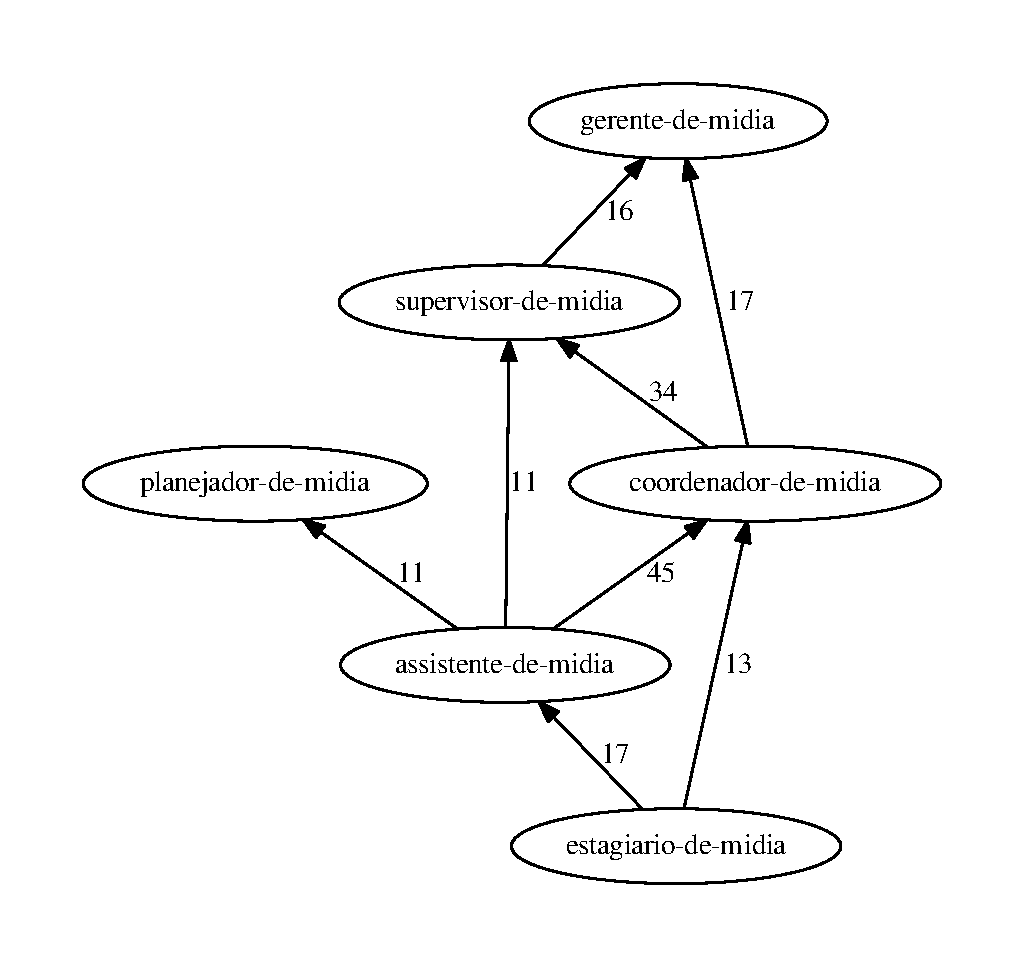
\includegraphics[scale=0.6]{cluster_23.pdf}
  \caption{Parte do Mapa de Carreiras}
  \label{fig:ex-mapa-midia}
\end{figure}

É possível observar parte do Mapa VAGAS de Carreiras (MCar) na Figura~\ref{fig:ex-mapa-midia} com as ocupações relacionadas à profissão de \enquote{mídia}. Nela, por exemplo, 16 pessoas passaram de \enquote{supervisor-de-midia} para a ocupação \enquote{gerente-de-midia}.

As ocupações no MCar foram definidas a partir de \textit{consenso} nos currículos. Como o título da ocupação é um campo em que o usuário digita livremente, assumiu-se que, se um grupo \enquote{suficientemente grande} de pessoas entra em acordo sobre uma certa nomenclatura, ela representa objetivamente uma ocupação~\cite{Gunz2007-hr}.

Uma das maiores dificuldades está em se definir o quanto um consenso precisa ser \enquote{suficientemente grande} para de fato existir uma ocupação. Para os fins desse trabalho, esse número foi obtido de forma experimental e empírica. Para isso, procurou-se o número mínimo de repetições exatas na grafia das ocupações de maneira não fossem encontrados erros de digitação recorrentes. Esse número é atualmente 30 repetições, ou 10 transições com exatamente a mesma grafia em ambos os lados da transição.

Para a criação do MCar foram usados os currículos anonimizados de 10 milhões de usuários registrados no site VAGAS.com.br. A seleção de dados, bem como o processamento das informações, seguiu um procedimento conservador. Isso significa que as decisões tomadas em sua construção procuram minimizar os erros decorrentes da qualidade dos dados, mesmo que isso signifique trabalhar com uma quantidade menor de dados.

Da massa de currículos, apenas os atualizados no período entre 2011 e 2016 foram usados. Currículos em duplicação foram removidos usando o CPF como identificador, em caso de duplicação, apenas o currículo mais recente foi considerado. Na impossibilidade de se verificar a duplicação, como por exemplo, na ausência do CPF, o currículo também foi descartado.

Finalmente, algumas informações gerais foram extraídas dos currículos que sobreviveram ao processo acima e o restante das informações foi descartada, incluindo quaisquer maneiras de se identificar a pessoa descrita no currículo.

A informações extraídas são o sexo, último salário, graduação (se existente) ou escolaridade, e a sequência de ocupações pelo qual o profissional passou com o título, descrição e período em que exerceu a ocupação.

O título da ocupação é um dos principais artefatos do MCar, é ele quem fornece a identidade para o nó. Como descrito acima, nos currículos, o título da ocupação é um campo de texto livre, ou seja, o usuário pode digitar o título sem restrições. Se por um lado isso permite a inserção de ocupações de nicho, novas ou que usem jargão de área; também significa que os títulos possuem erros de grafia, variações de gênero (como em \enquote{advogado} e \enquote{advogada} ou \enquote{moto boy} e \enquote{moto girl}), composição de múltiplas ocupações em um mesmo título (como \enquote{caixa / balconista}), abreviações e toda sorte de erros de interpretação possíveis.

As ocupações passam por um corretor ortográfico criado especificamente para esse trabalho, uma vez que um corretor tradicional não é capaz de identificar jargões de área como \enquote{enfermeiranda}, \enquote{rigger} ou \enquote{IRLA}.

Como exemplo, o dicionário do corretor possui cerca de 750 variações ortográficas que são traduzidas para o termo \enquote{auxiliar}, dentre eles, simples erros de omissão como \enquote{uxiliar} até variações mais elaboradas como \enquote{ausciliar} e \enquote{alsilia}.

Após o trabalho de correção ortográfica, os títulos foram agrupados e contados. Especialistas da empresa verificaram os resultados dos maiores grupos para identificar anomalias como os títulos \enquote{sim}, \enquote{não} e \enquote{o mesmo}, essas ocupações foram excluídas do trabalho.

Finalmente, pares de ocupações foram gerados. Por exemplo, um currículo com a sequência de ocupações \enquote{saladeiro} $\to$ \enquote{chapeiro} $\to$ \enquote{cozinheiro} gera os pares \enquote{saladeiro} $\to$ \enquote{chapeiro} e \enquote{chapeiro} $\to$ \enquote{cozinheiro}.

Os pares foram agrupados para formar o peso de cada conexão na rede final. O peso mínimo 10 foi definido empiricamente para que sejam removidas do mapa as movimentações que incluem erros que o corretor ortográfico não foi capaz de detectar.

Nesse ponto do processo, cerca de 23 milhões de ocupações dos currículos foram agrupadas em aproximadamente 8 mil ocupações distintas.

Finalmente, os pares de ocupações foram conectado entre si a rede final foi construída e armazenada em um banco de dados de grafo. Um sistema online (disponível em http://www.vagas.com.br/mapa-de-carreiras) disponibiliza as informações publicamente.

Apesar de gratuito, os dados do Mapa VAGAS da Carreira não são de uso livre. A empresa gentilmente cedeu os dados ao pesquisador para esse trabalho.

%===================================
\section{Detecção de Comunidades}
%===================================

Uma comunidade é um subgrafo com conexões mais \textit{coesas} entre seus nós do que com nós do restante do grafo. A palavra \enquote{coesão} aqui pode ser interpretada de várias maneiras. Para \citeonline{Ahn2010-uh,Evans2009-lq,Newman2004-jg}, uma comunidade é definida quando o número de conexões internas do subgrafo é maior que o número de conexões que o conecta ao resto do grafo, ou quando uma comunidade possui um densidade de conexões mais alta do que o esperado em uma rede aleatória equivalente. De qualquer forma, para esses autores, o número de conexões é o fator determinante para a identificação da comunidade.

\citeonline{Rosvall2009-sd,Van_Dongen2000-qm}, por sua vez, trabalham a detecção de comunidades como a identificação de fluxos mais frequentes na rede. Assumindo que uma conexão representa um fluxo, comunidades possuem fluxo maior entre seus nós do que com nós fora da comunidade.

Essas abordagens distintas são aplicáveis a cenários diferentes. A densidade de conexões é mais adequada em redes onde a estrutura é importante, como por exemplo, em uma rede social. Já em redes que representam fluxos, com circuitos ou redes de transporte, a segunda abordagem é mais atraente~\cite{Rosvall2009-sd}.

Para esse trabalho, a identificação de comunidades por fluxo é adequada por concepção. Como explicado na Seção~\ref{sec:carreira}, as fronteiras de carreira são definidas pelo consenso das movimentações profissionais: transições menos frequentes definem as fronteiras.

Essa frequência é, obviamente, relativa ao fluxo entre os nós próximos, dez transições para uma ocupação como \enquote{Auxiliar Administrativo}, que possui dezenas de milhares de profissionais entrando e saindo, não tem a mesma importância que \enquote{Assistente de Mídia} (Figura~\ref{fig:ex-mapa-midia}), em que essa dezena representa mais de 10\% das transições registradas.

O algoritmo Infomap (detalhado na Seção~\ref{sec:infomap}) utiliza \textit{random walkers} para identificar comunidades. Os caminhos em que eles circulam mais frequentemente são considerados como fazendo parta da mesma comunidade, por outro lado, caminhos raramente utilizados definem as fronteiras entre uma comunidade e outra, de maneira análoga à concepção de fronteiras de carreira de~\citeonline{Gunz2007-hr}.

Portanto, por concepção, a identificação de comunidades do algoritmo Infomap identifica fronteiras de carreiras em uma rede em que as conexões representam o fluxo de profissionais entre ocupações\footnote{Ronie: acho que dá para explicar melhor, e também acredito que esse ponto precisa ser provado (ou ao menos ter indícios), mas a linha de raciocínio é essa.}.

%===================================
\subsection{O Algoritmo Infomap} \label{sec:infomap}
%===================================

Segundo \citeonline{Grunwald2007-bt}, quaisquer regularidades em um conjunto de dados podem ser usadas para comprimi-los, ou seja, descrevê-los usando uma quantidade menor de símbolos. Quanto maior a regularidade, maior a compressão, dessa forma, dentre várias representações possíveis dos dados, a que apresentar maior compressão é também aquela que identifica melhor padrões nos dados. A Descrição de Comprimento Mínimo (\textit{Minimum Description Length}) é a disciplina que estuda essa relação.

O algoritmo Infomap aproveita essa dualidade entre detecção de padrões e compressão de dados para identificar padrões de fluxo em redes~\cite{Rosvall2009-sd}.

Para compreender o algoritmo, é preciso entender como o MDL pode ser usado para representar caminhos em uma rede.

Descreve-se o caminho que um \enquote{random walker} faz em uma rede através da sequência de nós pelo qual ele passa. Por exemplo, assumindo uma rede com os nós $A$, $B$ e $C$, um caminho possível poderia ser descrito por $ABACBA$.

Esse nós podem ser recodificados usando uma sequência binária, por exemplo, $A = 00$, $B = 01$ e $C = 10$. O caminho acima descrito seria representado, sem ambiguidades, pelos 12 bits: $000100100100$.

É possível representar esse mesmo caminho de maneira reduzida observando-se seus padrões. O nó $A$ aparece mais frequentemente no caminho que os nós $B$ e $C$, se a codificação usada para representar $A$ for menor do que a dos outros, a descrição do caminho também será menor. Nesse exemplo, usando-se a seguinte codificação $A = 0$, $B = 10$ e $C = 11$, o mesmo caminho pode ser representado, sem ambiguidades, pelos 9 bits: $010011100$.

Continua\ldots

%===================================
\section{Identificação de Carreiras no Mapa de Carreiras}
%===================================

%===================================
\section{Conclusões e Perspectivas Futuras}
%===================================

O fato de ocupações \enquote{ponte} ser encontrada predominantemente no início da carreira pode significar que depois de definido um caminho profissional a movimentação para outra carreira não é feita por movimentações pré-definidas, mas que cada movimentação dessas ocorre de maneira particular. Ao mesmo tempo, indica uma certa mobilidade de escolhas no princípio da carreira.

Os exemplos encontrados de ocupações homônimas indicam uma certa similaridade nas atribuições, mas em especialidades diferentes. TK

\newpage

\bibliography{main}
\end{document}
